% ==========================================================
% ENTREGA 1 — O corpus do projeto
% Projeto Integrador III — Motor de Busca — Ciência de Dados
% Fatec Baixada Santista – Rubens Lara
% Versão em .tex puro (sem R/knitr) do modelo entrega-1-corpus.Rnw.
% Todos os números foram calculados sobre corpus_pre_recorte.csv
% (224 documentos) e as buscas de teste seguem o busca_ri.R
% (BM25 com k1 = 1,2 e b = 0,75; TF-IDF com cosseno).
%
% Trechos em vermelho \revisar{...} são pontos que o grupo precisa
% confirmar ou preencher. Procure por "revisar" antes de entregar.
%
% COMPILAR: pdflatex -> bibtex -> pdflatex -> pdflatex
%           (ou: latexmk -pdf entrega-1-corpus.tex)
% ARQUIVOS NA MESMA PASTA: entrega-1-corpus.tex e referencias.bib
% REQUISITOS: LaTeX com abntex2 (texlive-publishers) e pgfplots.
% ==========================================================

\documentclass[
  article,
  12pt,
  oneside,
  a4paper,
  english,
  brazil
]{abntex2}

\usepackage[T1]{fontenc}
\usepackage[utf8]{inputenc}
\usepackage{lmodern}
\usepackage{amsmath,amssymb}
\usepackage{icomma}
\usepackage{booktabs}
\usepackage{xcolor}
\usepackage{pgfplots}
\pgfplotsset{compat=1.16}
\usepackage[alf]{abntex2cite}

\hypersetup{hidelinks}

% Marcador de pontos a revisar pelo grupo
\newcommand{\revisar}[1]{{\color{red}\textbf{[revisar: #1]}}}

% ----------------------------------------------------------
% DADOS DA ENTREGA
% ----------------------------------------------------------
\titulo{O corpus do projeto: parágrafos da Wikipédia sobre a Baixada Santista}
\tituloestrangeiro{}
\autor{{Grupo 3Mkt}}
\local{Santos-SP}
\data{\today}

\newcommand{\nomecurso}{Tecnologia em Ciência de Dados}
\newcommand{\nomedisciplina}{Projeto Integrador III --- Motor de Busca}
\newcommand{\nomeprofessor}{Prof.\ Dr.\ João Paulo Ferreira de Mello}
\newcommand{\repositorio}{3mkt-pi3}
\newcommand{\integrantes}{%
  João Pedro -- RA 0051352511002 \\
  Lucas Marques -- RA 0051352511024 \\
  Timóteo Blank -- RA 0051352511014%
}

\begin{document}

\selectlanguage{brazil}
\frenchspacing

\maketitle

\begin{center}
  \small
  Fatec Baixada Santista -- Rubens Lara \\
  \nomecurso{} \quad|\quad \nomedisciplina{} \quad|\quad \nomeprofessor{} \\[0.4em]
  \integrantes \\[0.4em]
  Repositório: \texttt{\repositorio}
\end{center}

\textual

% ==========================================================================
\section{Introdução}
% ==========================================================================

O tema deste motor de busca é a Baixada Santista: seus bairros, praias e
municípios, e a história e os problemas que os acompanham. Quem o usaria é
alguém de fora ou de dentro da região, como por exemplo um comprador de imóvel, um estudante,
uma família em busca de passeio, que tem uma dúvida concreta e quer o trecho
de texto que a responde, não uma lista de páginas. Em recuperação de
informação, o que se atende é a \emph{necessidade de informação} de alguém, não
a consulta literal; por isso as perguntas vêm antes
do corpus. O motor deve responder a três delas:

\begin{itemize}\itemsep0pt
  \item \textbf{q01}: ``Quero comprar uma casa e preciso saber se o Gonzaga é um
        lugar calmo para se viver.''
  \item \textbf{q02}: ``Vou fazer um trabalho sobre recuperação ambiental e
        quero entender se Cubatão ainda sofre com poluição industrial ou se o
        cenário melhorou.''
  \item \textbf{q03}: ``Quero levar minha família para um passeio cultural e
        preciso saber quais são os monumentos mais importantes sobre a fundação
        de São Vicente.''
\end{itemize}

Este texto apresenta a fonte escolhida, descreve como o corpus foi montado e
mostra, com evidência, até onde ele tem condição de responder a essas perguntas.

% ==========================================================================
\section{A fonte e o documento}
% ==========================================================================

O texto vem da Wikipédia (Wikimedia Foundation, 2026) em português, obtido pela API do
MediaWiki em texto puro, sob a licença CC BY-SA, com acesso em
11/09/2026. Foram pedidas 16 artigos: oito bairros de Santos
(Gonzaga, Boqueirão, Ponta da Praia, José Menino, Aparecida, Macuco, Vila
Mathias e Campo Grande), quatro praias (Tombo, Astúrias, Pitangueiras e
Gonzaga) e quatro municípios (Guarujá, São Vicente, Cubatão e Praia Grande).
Uma delas, Pitangueiras, não foi encontrada (Seção~3), restando 15 artigos. As perguntas saem
dos próprios artigos: Gonzaga para a q01, Cubatão para a q02 e São Vicente
para a q03; as demais são vizinhas que fazem o motor distinguir lugares que
compartilham vocabulário (\emph{praia}, \emph{bairro}, \emph{cidade}).

O documento é o {parágrafo}, identificado como \texttt{pagina-pN} (por
exemplo, \texttt{cubatao-p3}). Um parágrafo é a menor unidade que responde
sozinha a uma pergunta: o \texttt{cubatao-p3} diz que Cubatão foi a cidade mais
poluída do mundo e depois se recuperou, e isso basta para a q02. Com o artigo
inteiro como documento, o motor diria apenas ``a resposta está em Cubatão'',
sem apontar onde.

O corpus foi escolhido por a região ser conhecida pelos autores e porque a Wikipédia tem licença
livre, API estável e texto já em prosa.

% ==========================================================================
% ==========================================================================
\section{Como o corpus foi obtido}
% ==========================================================================

A coleta roda em R e segue seis passos. (1) Para cada título, uma função chama
a API da Wikipédia pedindo o texto puro, segue redirecionamentos, identifica o
projeto no \emph{user agent}, espera 1,5 s entre requisições e tenta até cinco
vezes com espera crescente; ela avisa quando a página não existe, está vazia
(menos de 50 caracteres) ou parece desambiguação. (2) Os títulos que falharam
são listados e descartados. (3) Os cabeçalhos de seção (\texttt{== ... ==}) são
removidos. (4) O texto é dividido nas quebras de linha, e cada parágrafo recebe
o identificador do artigo mais seu número. (5) Um filtro mantém só parágrafos
com pelo menos 40 caracteres e algum caractere alfanumérico; o limiar de 40
foi escolhido para eliminar títulos residuais e rótulos como ``Ver também''.
(6) O resultado original rendeu 224 parágrafos. Entretanto, após a limpeza
manual e remoção de duplicatas exatas, tabelas demográficas soltas e dados
ruidosos, 30 linhas de dados foram excluídas. O arquivo consolidado
(\texttt{corpus.csv}) preservou a padronização e qualidade, resultando em
exatos 194 parágrafos válidos.

% ==========================================================================
\section{Defesa do corpus}
% ==========================================================================

As Tabelas~\ref{tab:diag} e~\ref{tab:origem} resumem o corpus atualizado após
a limpeza dos ruídos e remoção das duplicatas.

\begin{table}[htb]
  \centering
  \caption{Diagnóstico do corpus}
  \label{tab:diag}
  \small
  \begin{tabular}{@{}p{0.30\textwidth}p{0.62\textwidth}@{}}
    \toprule
    \textbf{Verificação} & \textbf{Resultado} \\
    \midrule
    Tamanho                 & $N = 194$ documentos de 12 páginas \\
    Tokens por documento    & 4 a 227 (média 65,7; mediana 55,5) \\
    Vocabulário bruto       & 4.371 termos distintos em 12.750 tokens \\
    Página que domina       & \texttt{Praia Grande (São Paulo)}: 51 de 194 (26,3\%) \\
    Documentos suspeitos    & 26 com menos de 20 tokens; nenhum com mais de 300 \\
    Sujeira                 & 189 com acento, 193 com pontuação, 135 com dígitos (de 194) \\
    \bottomrule
  \end{tabular}
  \fonte{Elaborada pelos autores a partir de \texttt{corpus.csv}.}
\end{table}

\begin{table}[htb]
  \centering
  \caption{Documentos por página de origem (tokens: média por documento)}
  \label{tab:origem}
  \footnotesize
  \begin{tabular}{@{}lrr@{\hspace{1.5em}}lrr@{}}
    \toprule
    \textbf{Página} & \textbf{Docs} & \textbf{Tokens} & \textbf{Página} & \textbf{Docs} & \textbf{Tokens} \\
    \midrule
    Praia Grande      & 51 & 68,5 & Ponta da Praia       & 6 & 47,3 \\
    Guarujá           & 41 & 71,2 & Praia das Astúrias   & 5 & 33,4 \\
    Cubatão           & 35 & 73,4 & Aparecida (Santos)   & 4 & 45,8 \\
    São Vicente       & 27 & 74,7 & Campo Grande (Santos)& 4 & 37,8 \\
    Boqueirão (Santos)&  8 & 37,6 & José Menino          & 4 & 43,8 \\
    Gonzaga (Santos)  &  7 & 49,9 & Praia do Tombo       & 2 & 71,5 \\
    \bottomrule
  \end{tabular}
  \fonte{Elaborada pelos autores.}
\end{table}

\textbf{Tamanho.} Os 194 documentos bastam para o julgamento da Aula 05. A faixa
é folgada, e o risco não é a falta de documentos, mas a qualidade deles, que
foi significativamente elevada com o filtro manual. Páginas inteiramente duplicadas
(como \texttt{Praia do Gonzaga}) e de listas sem prosa contínua foram expurgadas.

\textbf{Domínio de uma página.} Os quatro municípios somam 154 dos 194
documentos (79,4\%), e Praia Grande sozinha, 26,3\%. Um
município tem muito mais a dizer que um bairro, mas desequilibra o corpus:
o Gonzaga tem apenas sete documentos próprios contra 51 de Praia Grande. Como as
perguntas citam o lugar pelo nome, o desequilíbrio pesa menos, e a correção é
acrescentar mais páginas dos bairros (como a orla e o Centro Histórico) no futuro.

\textbf{Documentos que não são prosa.} Os 26 documentos curtos restantes representam
sentenças curtas porém informativas (descrições objetivas). Não há documentos longos 
demais (o maior tem 227 tokens), como mostra a Figura~\ref{fig:tam}.

\begin{figure}[htb]
  \centering
  \caption{Tokens por documento (194 documentos)}
  \label{fig:tam}
  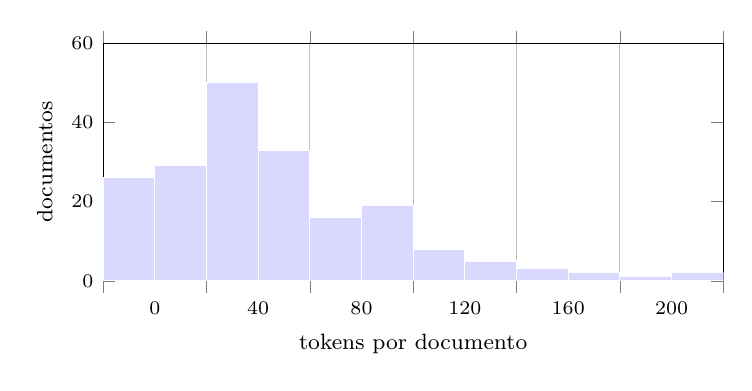
\begin{tikzpicture}
    \begin{axis}[
      ybar interval, width=0.78\linewidth, height=4.6cm,
      xlabel={tokens por documento}, ylabel={documentos},
      xmin=0, xmax=240, ymin=0, ymax=60, xtick={0,40,80,120,160,200,240},
      tick label style={font=\scriptsize}, label style={font=\footnotesize},
      ]
      \addplot[fill=blue!15, draw=white] coordinates {
        (0,26) (20,29) (40,50) (60,33) (80,16) (100,19) (120,8)
        (140,5) (160,3) (180,2) (200,1) (220,2) (240,0)
      };
    \end{axis}
  \end{tikzpicture}
  \fonte{Elaborada pelos autores.}
\end{figure}

\textbf{Sujeira.} Quase todos os documentos têm acento (189), pontuação (193)
ou dígitos (135). Isso é esperado e preserva a precisão das informações. O 
\texttt{busca\_ri.R} normaliza tudo (minúsculas, sem acentos, só letras e números)
e remove as palavras funcionais, o que reduz o vocabulário bruto de 4.371 para
cerca de 3.360 termos limpos e representativos.

\textbf{Os termos mais frequentes} no texto bruto são \texttt{de}, \texttt{a},
\texttt{e}, \texttt{o}, \texttt{do}, \texttt{da}, \texttt{em}, \texttt{que},
\texttt{com} e \texttt{na}: nenhum diz algo sobre o tema. Depois da limpeza
aparecem \texttt{sao}, \texttt{praia}, \texttt{cidade}, \texttt{vicente} e
\texttt{grande}, que descrevem perfeitamente a região.

\textbf{Veredito.} Foram rodadas as três perguntas no \texttt{busca\_ri.R}, com busca
vetorial (TF-IDF e cosseno) e BM25; a Tabela~\ref{tab:busca}
mostra o melhor documento de cada método.

\begin{table}[htb]
  \centering
  \caption{Melhor documento de cada pergunta e se ele responde}
  \label{tab:busca}
  \footnotesize
  \begin{tabular}{@{}p{0.06\textwidth}p{0.20\textwidth}p{0.20\textwidth}p{0.42\textwidth}@{}}
    \toprule
    \textbf{Perg.} & \textbf{BM25} & \textbf{Vetorial} & \textbf{O corpus responde?} \\
    \midrule
    q01 & \texttt{gonzaga-santos-p3} & \texttt{gonzaga-santos-p1} &
      \textbf{Não.} Os documentos do bairro tratam de comércio, shoppings e
      lazer; os indícios apontam exatamente o contrário de calma. \\
    q02 & \texttt{cubatao-p3} & \texttt{cubatao-p3} &
      \textbf{Em parte.} Traz a poluição dos anos 1980 e a recuperação (título da
      ONU, 1992), mas falta contexto extenso sobre o cenário atual. \\
    q03 & \texttt{sao-vicente-sao-
    paulo-p4} & \texttt{sao-vicente-sao-
    paulo-p4} &
      \textbf{Sim.} Cita a Casa de Taipa, a Igreja Matriz, o Engenho dos Erasmos,
      a Biquinha de Anchieta, a Ponte Pênsil e a encenação da fundação. \\
    \bottomrule
  \end{tabular}
  \fonte{Elaborada pelos autores, com \texttt{busca\_ri.R}.}
\end{table}

Os dois métodos concordam no primeiro resultado das três perguntas, o que dá
confiança de que o achado vem de fato do corpus, não do método. A q03 é bem atendida; a
q02 só responde à parte histórica da recuperação; e a q01 revela uma lacuna: a 
Wikipédia descreve o Gonzaga estritamente como polo comercial. O descarte das duplicadas 
funcionou perfeitamente: os textos idênticos que existiam sob ``Praia do Gonzaga'' foram 
expurgados, enxugando o espaço de busca sem prejudicar os documentos originais 
de ``Gonzaga (Santos)'', que dominaram o ranking. Para a q01, os autores deveriam 
acrescentar páginas com perfil mais residencial.


% ----------------------------------------------------------
% REFERÊNCIAS
% ----------------------------------------------------------
\postextual
\bibliography{referencias}
Wikimedia Foundation, 2026
\end{document}